\paragraph{Sơ đồ tuần tự Luồng Tải lên tài liệu cá nhân}

Luồng này mô tả quá trình người dùng tải lên tài liệu cá nhân. Document Service kiểm tra subscription khi không chạy ở môi trường \texttt{development}, validate file, lưu metadata, upload file gốc lên Cloudflare R2 và gửi task xử lý nền qua Celery/RabbitMQ.

\begin{figure}[H]
\centering
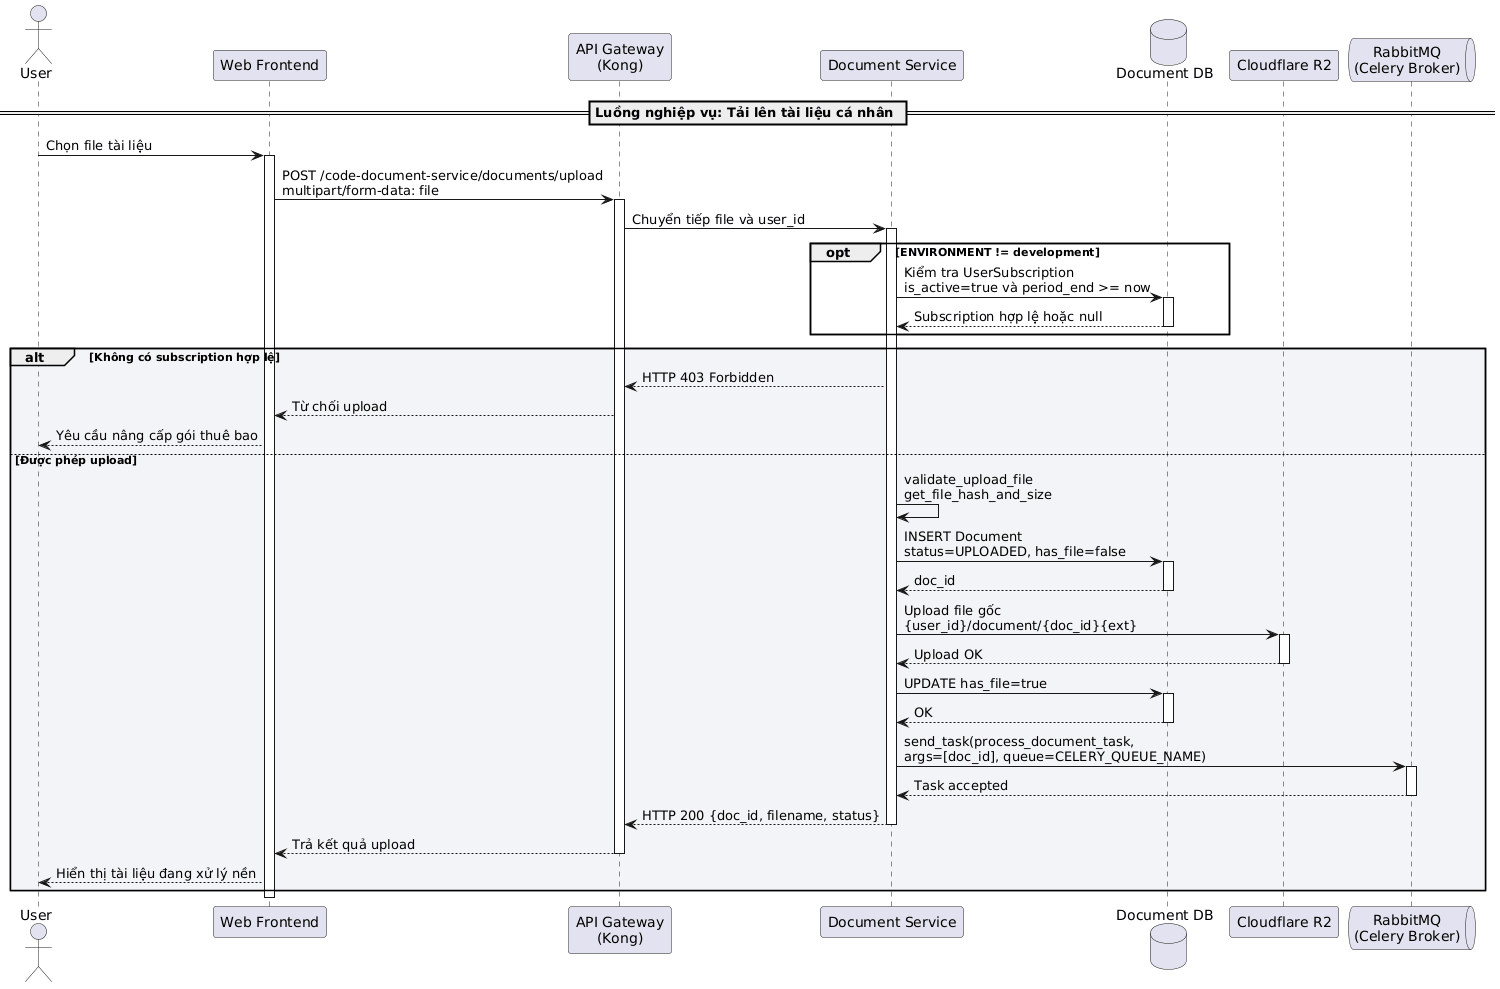
\includegraphics[scale = 0.18]{contents/Sequence/UML-Sequence-UserUploadPersonalDocument.png}
\caption{Sơ đồ tuần tự Luồng Tải lên tài liệu cá nhân}
\end{figure}

\subparagraph{Các thành phần tham gia}

\begin{table}[H]
\centering
\renewcommand{\arraystretch}{1.3}
\begin{tabular}{|l|l|p{5cm}|}
\hline
\textbf{Thành phần} & \textbf{Phân loại} & \textbf{Vai trò trong hệ thống} \\ \hline
User & Actor & Người dùng tải lên tài liệu cá nhân. \\ \hline
Web Frontend & Component & Giao diện web Next.js. \\ \hline %%%% Component & Gọi \texttt{documentService.uploadDocument} bằng multipart form data. \\ \hline
API Gateway (Kong) & Component & Cổng API chuyển tiếp các yêu cầu API. \\ \hline %%%% Component & Định tuyến request tới Document Service. \\ \hline
Document Service & Microservice & Kiểm tra quyền, validate file, lưu metadata và publish task xử lý nền. \\ \hline
Document Database & Database & Lưu Document và bảng \texttt{user\_subscriptions}. \\ \hline
Cloudflare R2 & Object Storage & Lưu file gốc của người dùng. \\ \hline
RabbitMQ & Message Broker & Nhận Celery task \texttt{process\_document\_task}. \\ \hline
\end{tabular}
\caption{Các thành phần tham gia luồng tải lên tài liệu cá nhân}
\end{table}

\subparagraph{Mô tả tổng quan}
\begin{itemize}
\item Web Frontend gọi \texttt{POST /code-document-service/documents/upload} với multipart file.
\item Document Service kiểm tra \texttt{UserSubscription.is\_active=true} và \texttt{period\_end >= now} khi môi trường khác \texttt{development}.
\item File được validate, tính hash/size và tạo bản ghi Document với \texttt{status=UPLOADED}, \texttt{has\_file=false}.
\item File gốc được upload lên R2 theo đường dẫn \texttt{\{user\_id\}/document/\{doc\_id\}\{ext\}}, sau đó cập nhật \texttt{has\_file=true}.
\item Service gửi Celery task \texttt{process\_document\_task(doc\_id)} vào \texttt{CELERY\_QUEUE\_NAME} để xử lý tài liệu trong nền.
\end{itemize}
